\chapter{More Interactivity and Dynamic Views}

\section{Introduction}
...To be filled...

\section{More on Event Handlers}
In this section we will explore more about event handlers. We will also see numerous ways to create them and hook them to the widgets.

\subsection{Create New Project}
\label{sec:createProj}

Create a new project from scratch. Perform the following steps:
\begin{enumerate}
	\item Create a new project having name ``\texttt{Lec5}''
	\item Select minimum API 16 : Android 4.1 (Jelly Bean).
	\item Select ``\texttt{Empty Activity}''
	\item Accept default values for activity and click finish. \\
\end{enumerate}

\subsection{Adding Event Handlers outside Java Code}
Modify \texttt{activity\_main.xml} layout so that it has four buttons on it and label them according to the following figure. Also set their \texttt{id's} as shown in the ``component tree'' on the right side. Note that the root element is set to \texttt{LinearLayout}:

\begin{center}
	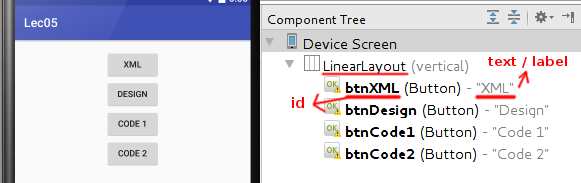
\includegraphics[scale=0.4]{chapters/ch05/images/1}
\end{center}

Event handlers are callback functions in your code that handle a particular event such as a user click or timer expire etc. There are a few ways to ``attach'' event handlers (also known as ``callback listeners'') to the views. Let's look at various ways to do that:

\subsubsection{Through Layout XML Code}
We've already seen this method in previous lecture (please refer to lecture 4 notes, section 3.6 for more details). To recap, this is one of the easiest methods to attach an event listener to a view. 

Open up \texttt{activity\_main.xml} and switch to the text mode. Find the \texttt{<Button>} tag having text ``\texttt{XML}'' and id ``\texttt{btnXML}''. Add an \texttt{onClick} attribute and name it \texttt{onBtnXMLClicked} (line number 19 shown below):

\begin{center}
	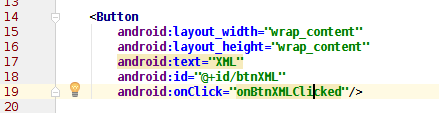
\includegraphics[scale=0.4]{chapters/ch05/images/2}
\end{center}

Bring the keyboard cursor on the \texttt{onBtnXMLClicked} string literal. A yellow bulb will appear on the left side. Click it and select ``Create in `onBtnXMLClicked(View)' MainActivity'':

\begin{center}
	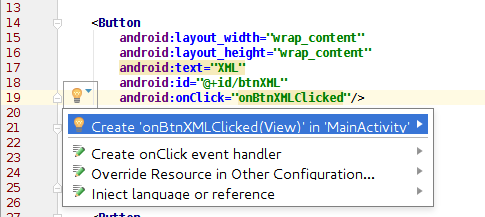
\includegraphics[scale=0.4]{chapters/ch05/images/3}
\end{center}

This will automatically create an event handler method and link it to the button. Go to \texttt{MainActivity.java} and you'll see the method created in the \texttt{MainActivity} class. Whenever you click the button this method will be executed:

\begin{center}
	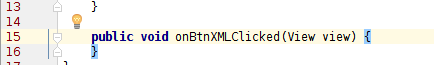
\includegraphics[scale=0.4]{chapters/ch05/images/4}
\end{center}

Go ahead and add a log message in it, or a \texttt{Toast} if you are feeling adventurous.
You can find more about toasts \href{https://developer.android.com/guide/topics/ui/notifiers/toasts.html}{here}. Run the app on a device or emulator to see if the \texttt{XML} button is working.

\subsubsection{Through Layout Design Mode}
Let's implement the second button labeled ``Design''. Open up \texttt{MainActivity.java} and \textit{manually} add the following function (your line numbers may be different). Notice that the name of the function is greyed out. This is because we haven't hooked it to any view (button in our case) yet:

\begin{center}
	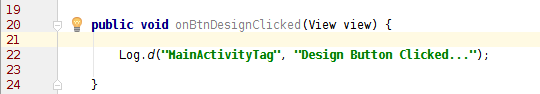
\includegraphics[scale=0.4]{chapters/ch05/images/5}
\end{center}

Event listener functions MUST have exactly the same signature as shown above. Please refer to Lecture 4 notes, section 3.6 for more details about function signatures. \\

Now switch to the design mode. Make sure that you've selected ``Design'' button. Go to the properties panel and in the \texttt{onClick} attribute add the name of the method we are trying to hook i.e: \texttt{onBtnDesignClicked}:

\begin{center}
	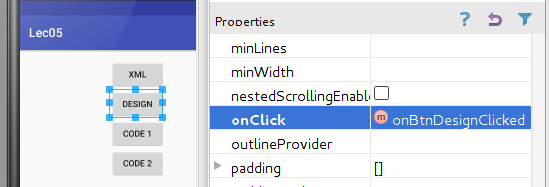
\includegraphics[scale=0.4]{chapters/ch05/images/6}
\end{center}

When you run the app you will see the correct message printed on the console when you click the ``Design'' button. For more information about Log messages please refer to Lecture 4 notes section 3.3.

\subsection{Adding Event Handlers from Java Code}
\subsubsection{Anonymous Inner Classes}
\label{sec:anonInnerClass}

\textit{This is a very important section, please read it very carefully and make sure that you've understood everything. Read it multiple times if you have to!} \\

In java the functions are NOT first class. This means that you can't pass functions as parameters or return functions from other functions. You can't even have references to the functions. Unlike C++, there is no concept of a function pointer in Java. This means that you can't do the following:

\begin{verbatim}
public void MyFunction(){
    ...
}

someObj.SomeFunction(MyFunction); // <-- WRONG !!!
OR
someObj.memberVar = MyFunction;   // <-- WRONG !!!
\end{verbatim}

But this means trouble! Then how do we attach event listener functions to the view objects? It appears that there is a way. We can't have references to functions and we can't pass functions as parameters to other functions. But we CAN pass objects as parameters to other functions! So we can exploit this fact and do the following: 

\begin{quote}
	\textit{Instead of trying to pass a function into the parameter, wrap that function inside of an object and then pass that object as a parameter instead.}
\end{quote}

Pseudo-code is given below:

\begin{verbatim}
interface BaseClass{
    public void MyFunction();
}
class MyNewClass implements BaseClass{
    @override public void MyFunction(){
        ...
    }
}
BaseClass myObj = new MyNewClass();
someObj.SomeFunction(myObj); // <-- CORRECT !!!
OR
someObj.memberVar = myObj;   // <-- CORRECT !!!
\end{verbatim}

This is called the ``Command Design pattern''. You can learn more about this design pattern by clicking \href{https://en.wikipedia.org/wiki/Command\_pattern}{here}.\\

There is an interface having a single function in android called ``\texttt{OnClickListener}''. You need to inherit and override this interface and then you can pass that object as parameters which includes the ``\texttt{onClick()}'' method. You can view more details \href{http://developer.android.com/reference/android/view/View.OnClickListener.html}{here}. \\

To summerize, this is what you need to do:
\begin{enumerate}
	\item Extend \texttt{View.OnClickListener} and override \texttt{onClick} method.
	\item Create an object of that child class and pass it as parameter to the view to attach event listener:
	\begin{verbatim}
	class MyNewClass implements OnClickListener{
	@override public void onClick(View view){
	...
	}
	}
	OnClickListener mylistener = new MyNewClass();
	button.setOnClickListener(mylistener); // <-- CORRECT !
	\end{verbatim}
	
\end{enumerate}

\vskip 3mm
But instead of defining a new class (\texttt{MyNewClass} in this case), \textit{java provides special syntax which allows us to declare and instantiate a class at the same time}, called the ``Anonymous Inner Class''. Unlike the regular class syntax, anonymous inner class syntax is an expression. \textit{This is a nameless or throw-away class that you declare right where you want to use it.} For example, above code would become (and is exactly the same as) following:

\begin{verbatim}
OnClickListener mylistener = new OnClickListener{
@override public void onClick(View view){ 
... 
} 
};
button.setOnClickListener(mylistener);
\end{verbatim}

Or alternatively you can even skip the extra variable and create anonymous inner right inside the parameters:

\begin{verbatim}
button.setOnClickListener(new OnClickListener{
@override public void onClick(View view){ 
... 
} 
});
\end{verbatim}

View more on Anonymous Inner Classes \href{https://docs.oracle.com/javase/tutorial/java/javaOO/anonymousclasses.html}{here}.

\subsubsection{Through Java Code: Method 1}
Armed with new knowledge now we are ready to add event listeners to ANY view object. \\

Open up \texttt{MainActivity.java} and go to the \texttt{onCreate} function. Add the code shown in following figure from lines 16 to 23: 

\begin{center}
	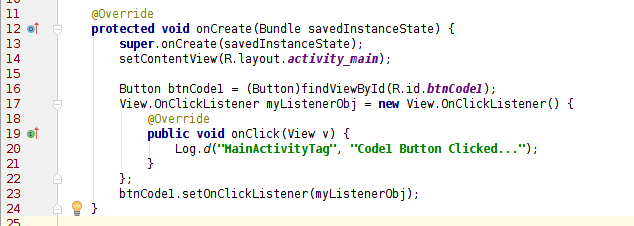
\includegraphics[scale=0.4]{chapters/ch05/images/7}
\end{center}

\begin{itemize}
	\item \textit{Line 16:} First we get the reference of button having id ``\texttt{btnCode1}'' and text label ``Code1''.
	\item \textit{Line 17-22:} Here we create a listener object. If you don't understand this then please refer to the ``anonymous inner classes'' section \ref{sec:anonInnerClass} of this document. IMPORTANT: DO NOT forget the semi-colon at the end of line 22 !!!
	\item \textit{Line 23:} Finally we pass the listener object through button's \texttt{setOnClickListener} method. When this button is clicked the listener object's \texttt{onClick} method will be executed.
\end{itemize}

\begin{quote}
	\textit{``TIP: You can use the same listener object on many views. However you would have to detect the view ids inside the \texttt{onCLick} function in order to know which view got clicked''.}
\end{quote}

Let's add event listener to the last button! Go to line 25 and add the following lines of code (lines 25-31). Notice that this time we are declaring the anonymous inner class right inside the function parenthesis (a bit of short-cut to the above code):

\begin{center}
	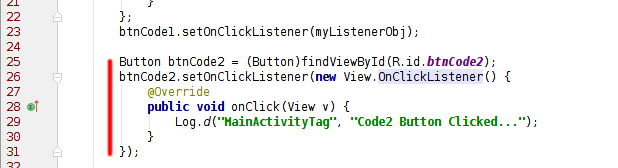
\includegraphics[scale=0.4]{chapters/ch05/images/8}
\end{center}

Run the app and make sure that all of the buttons are working properly.

\begin{quote}
	\textit{``There are advantages of using anonymous inner classes. You can attach listeners at run-time (as opposed to xml layouts where it must be done at compile time). You can attach as many event listeners to as many views as you like WITHOUT ever defining new member function inside the \texttt{MainActivity} or any other class! This method has its disadvantages though, one is the possibility of code repetition, but that is relatively rare.''}
\end{quote}

\subsubsection{Through Java Code: Method 2}
Now we will see another method to hook event listeners to the views. General idea is to inherit the main activity class from \texttt{View.OnClickListener} interface and then override the \texttt{onClick} virtual function to catch any click events. \\

Inherit the \texttt{MainActivity} class from \texttt{View.OnClickListener} interface. This will turn your main activity class into a big huge listener object which you can pass into the function parameters!!!

\begin{center}
	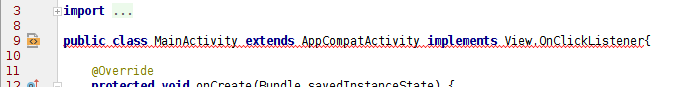
\includegraphics[scale=0.4]{chapters/ch05/images/9}
\end{center}

The project can't compile yet because we must implement ALL the interface methods! The \texttt{View.OnClickListener} interface contains only a single abstract method \texttt{onCreate} that we must override.You can learn more about the \texttt{View.OnClickListener} interface \href{http://developer.android.com/reference/android/view/View.OnClickListener.html}{here}.\\

Right click anywhere inside \texttt{MainActivity} class and select ``Generate'' or press ``Alt + Insert''. A little menu will pop up. Select ``Override Methods''. Then a dialog box with huge amount of interfaces with all the abstract methods will open up. You may have to collapse some of the items. Roughly near the bottom there will be our desired interface \texttt{android.view.View.OnCLickListener} having an \texttt{onCLick} method underneath it. 

\begin{center}
	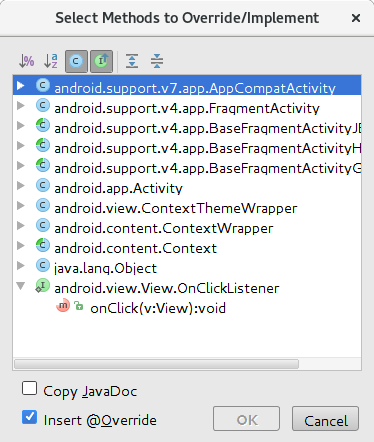
\includegraphics[scale=0.4]{chapters/ch05/images/10}
\end{center}

Click on the \texttt{onCLick} method and hit OK. A new method named \texttt{onCLick} will be created inside the \texttt{MainActicity} class by the android studio:

\begin{center}
	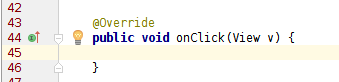
\includegraphics[scale=0.4]{chapters/ch05/images/11}
\end{center}

This class can now function as a listener object on its own. We will exploit exactly this fact. Remember that we created new listener objects and passed into the \texttt{setOnClickListener} method? Now we will just pass \texttt{MainActicity} as the listener object.

Go to the onCreate method and delete all the code from previous tasks that we wrote, bringing the method back to its original shape as follows:

\begin{center}
	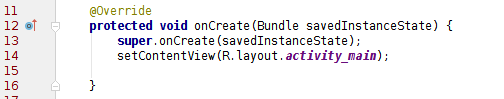
\includegraphics[scale=0.4]{chapters/ch05/images/12}
\end{center}

Inside \texttt{onCreate} Method, get reference to the buttons and add event listener by passing ``\texttt{this}'' as the listener object! (Specially note lines 17 and 20):

\begin{center}
	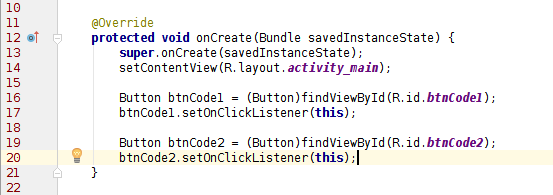
\includegraphics[scale=0.4]{chapters/ch05/images/13}
\end{center}

Almost done! Finally go to the \texttt{onClick} method. Since in this section we are passing ``\texttt{this}'' to every view as the listener object. When ever any view is clicked, the \texttt{onClick} method of the \texttt{MainActivity} class will be called: 

\begin{center}
	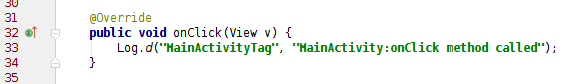
\includegraphics[scale=0.4]{chapters/ch05/images/14}
\end{center}

Run your app and try clicking the buttons and see what messages you get on the console.

\begin{quote}
	\textbf{Pop Quiz:} Why are we passing ``\texttt{this}'' as a parameter to the set listener method?
\end{quote}

\subsubsection{Exercise}

You have to write code inside the \texttt{onClick} method shown above and properly handle both the Code 1 and 2 buttons. (SPOILER: Solution is given on the next page!)

\newpage

\textbf{Solution:}
\begin{center}
	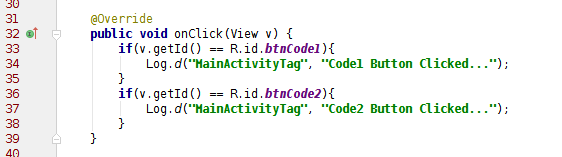
\includegraphics[scale=0.4]{chapters/ch05/images/15}
\end{center}

\vskip 3mm
You can mix and match any of the methods (1,2,3,4) described above in any combination you like.

\section{Dynamic Views}
Let's start fresh. Create a new project (follow section \ref{sec:createProj}). Name your project as \texttt{Lec5b}.

Any widget or a view or a view group that you can add through XML or the design mode you can add purely through programming. Every single field for every single view that you can change in design mode, you can also change through code. Every widget has a corresponding java class that we can use to instantiate and display the widget on the screen through code. It is entirely possible to create very complex layouts completely inside java code. \\

\subsection{Setting up the Layout file}
From your \texttt{activity\_main.xml} layout file, delete the default \texttt{TextView} and change the layout from Relative to Linear (vertical): \textbf{EXTREMELY IMPORTANT}: You must also set the id for this view. In this example we set it to ``\texttt{idLinearLayout}'' (line 11). Everything being referred from the code must have a ``Unique'' identifier:

\begin{center}
	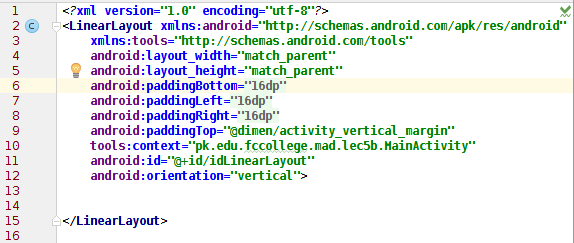
\includegraphics[scale=0.4]{chapters/ch05/images/16}
\end{center}

\begin{quote}
	Tip: You can specify any view's id from the design mode. You can also specify the id directly into the XML code. But when mentioning in the XML code the id must have a prefix ``\texttt{@+id/}'' (line 11 above).
\end{quote}

And that's it for the XML file. We won't be referring to it anymore.

\subsection{Adding views dynamically}
\label{sec:addViewsDynamically}
Remember that every activity must have a view group as a parent? Let's get the reference to the parent linear layout view group in our code. The java class for linear layout is ``\texttt{LinearLayout}''. But first create a member variable of type ``\texttt{LinearLayout}'' in the \texttt{MainActivity} class (line 9):

\begin{center}
	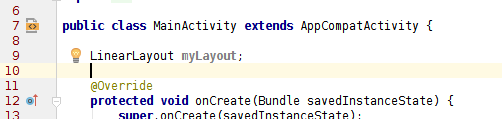
\includegraphics[scale=0.4]{chapters/ch05/images/17}
\end{center}

Now go to the \texttt{onCreate} function and get the reference to root linear layout view group object. Also setting its orientation to ``Vertical'' (lines 16, 17):

\begin{center}
	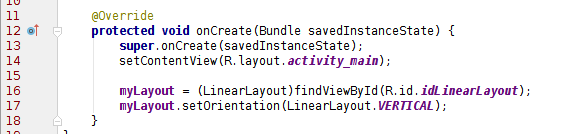
\includegraphics[scale=0.4]{chapters/ch05/images/18}
\end{center}

Note that we are using java code to set all the attributes of a view object. Let's add a simple button inside this layout. As you may've guessed, the java class for a button widget is ``\texttt{Button}''. Add lines 20 and 21 inside the \texttt{onCreate} function:

\begin{center}
	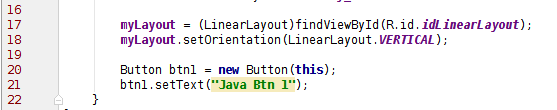
\includegraphics[scale=0.4]{chapters/ch05/images/19}
\end{center}

If you run the code, blank screen appears. Oh! We forgot to actually add the button to the layout, let's do that now. Add line 23:

\begin{center}
	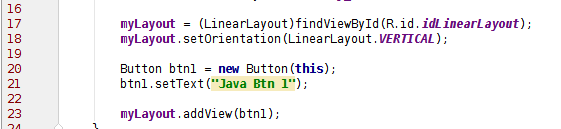
\includegraphics[scale=0.4]{chapters/ch05/images/20}
\end{center}

\vskip 3mm
\begin{quote}
	\textit{Notice that only view groups can add views as children. The button class doesn't even have ``\texttt{addView}'' method!}
\end{quote}

Run the code again and you will see a very wide button:

\begin{center}
	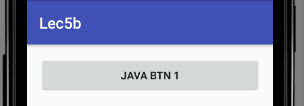
\includegraphics[scale=0.4]{chapters/ch05/images/21}
\end{center}

You can easily align the button text to left or right by changing its gravity fields. Notice the addition of line number 23 in the following snippet. You can combine multiple options using the \texttt{OR} operator `\texttt{|}':

\begin{center}
	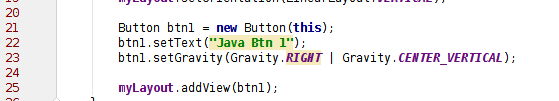
\includegraphics[scale=0.4]{chapters/ch05/images/22}
\end{center}

When you run the app, you will see the button text adjusting itself to the right side:

\begin{center}
	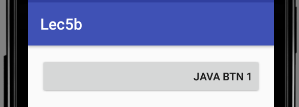
\includegraphics[scale=0.4]{chapters/ch05/images/23}
\end{center}

Ok maybe the button is too wide. Let's change its width to say ``\texttt{wrap\_content}''. Oops, it appears that we don't have any \texttt{width} member variable or \texttt{setWidth} method for button class. The solution is to use the ``\texttt{LayoutParams}'' class (nested under \texttt{LinearLayout}). This class contains fields like width, height, layout gravity, weight etc that we can fill in and pass into our desired view object. Lines 25 to 27 are setting width and height. Line 28 is setting ``\texttt{layout:gravity}'' (not just gravity) to right aligned. Finally in line 29 we pass the layout parameters to our button object:

\begin{center}
	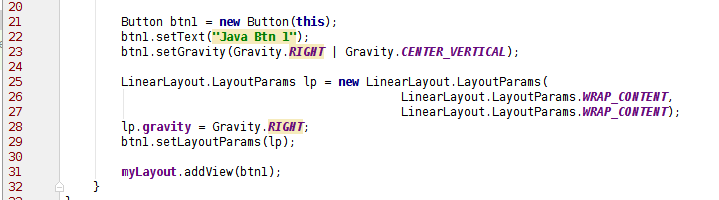
\includegraphics[scale=0.4]{chapters/ch05/images/24}
\end{center}

Run the program and you should get the following output:

\begin{center}
	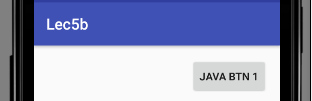
\includegraphics[scale=0.4]{chapters/ch05/images/25}
\end{center}

\vskip 3mm
Since the button was created through code \texttt{R.id.blahblah} doesn't work here. You must manually assign it a unique id (a unique integer number). (Line 33). \textit{As a programmer it is fully your responsibility to make sure that every single dynamically created object has a unique id}. Add \texttt{onClick} listener to this button object (lines 34 to 39. Listener functions are also discussed in detail in section 2.3.2):

\begin{center}
	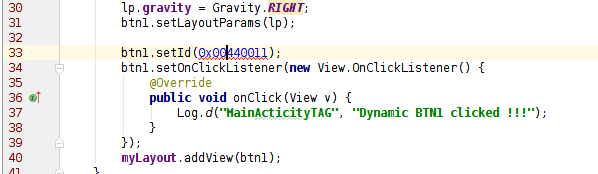
\includegraphics[scale=0.4]{chapters/ch05/images/26}
\end{center}

If you run the program you should see the correct output whenever the button is clicked! \\

Let's now add five buttons dynamically inside our root linear layout. Add the following code inside the \texttt{onCreate} method after line 40:

\begin{center}
	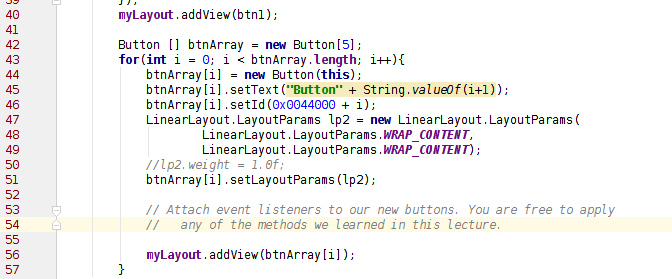
\includegraphics[scale=0.4]{chapters/ch05/images/27}
\end{center}

Run the app and you should see the following output:

\begin{center}
	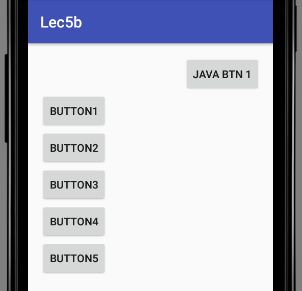
\includegraphics[scale=0.4]{chapters/ch05/images/28}
\end{center}

Un-comment line 50 in the above code and then see what happens.

\subsection{Inflators}
We've seen layout inflators in detail in Lecture 4 section 3.2. To simply put the job of an inflator is to read an xml description of the layout file and then create the views dynamically, just like we did above. You are now fully qualified to write your own layout inflator !!!

\section{Exercises}
\subsection{Exercise 1}
Modify the event listener for the very first button labeled ``\texttt{Java BTN1}''. Whenever this button is clicked, it should toggle between the HORIZONRAL and VERTICAL orientations of the root linear layout. \textit{Hint: We have already saved the reference to the root linear layout in a member variable named ``\texttt{myLayout}''}.

\subsection{Exercise 2}
Attach event listeners to these 5 buttons (replace lines 53,54 in the code snippet given on page number 12. Use an appropriate Method 1,2,3 or 4 as described in sections 2.3. Each button MUST display a Unique message upon clicking!

\subsection{Exercise 3}
Remember our previous class activity some lectures ago? Create the following layout \underline{completely through java code} (Your activity layout file should be completely empty, except for the root view group object):

\begin{center}
	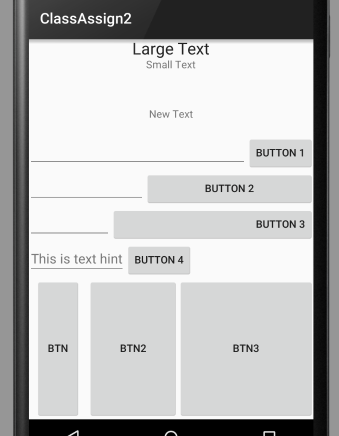
\includegraphics[scale=0.4]{chapters/ch05/images/29}
\end{center}

